\documentclass{beamer}
\usepackage[utf8]{inputenc}
\usetheme{Warsaw}

\title{Présentation du projet LSystemt}
\author{Augustin L\\ \and Luka K\\ \and Maël F\\ \and Paul M} 
\institute{Université de Caen Normandie\\
L2 Info\\ Groupe 4B}

\begin{document}

\begin{frame}
\titlepage
\end{frame}


\begin{frame}
\tableofcontents
\end{frame}


\section{Présentation du projet}

\subsection{Description générale du projet}

\begin{frame}

\begin{block}{Les objectifs du projet}
	\begin{itemize}
		\item \textbf{Développement d'un LSystem}
		\item Comprendre ce que sont les Systemes de Lindenmayer
		\item Projet codé à l'aide de contrats pour contrer les erreurs
		\item Développer un interpréteur de LSystem
		\item Développer une première interface en console
		\item Développer une interface 2D
		\item Développer une interface 3D
	\end{itemize}
\end{block}

\end{frame}



\subsection{Objectif du projet}

\begin{frame}
%
\begin{exampleblock}{Exemple de rendu finale en 2D/3D}

	\begin{figure}[h]
	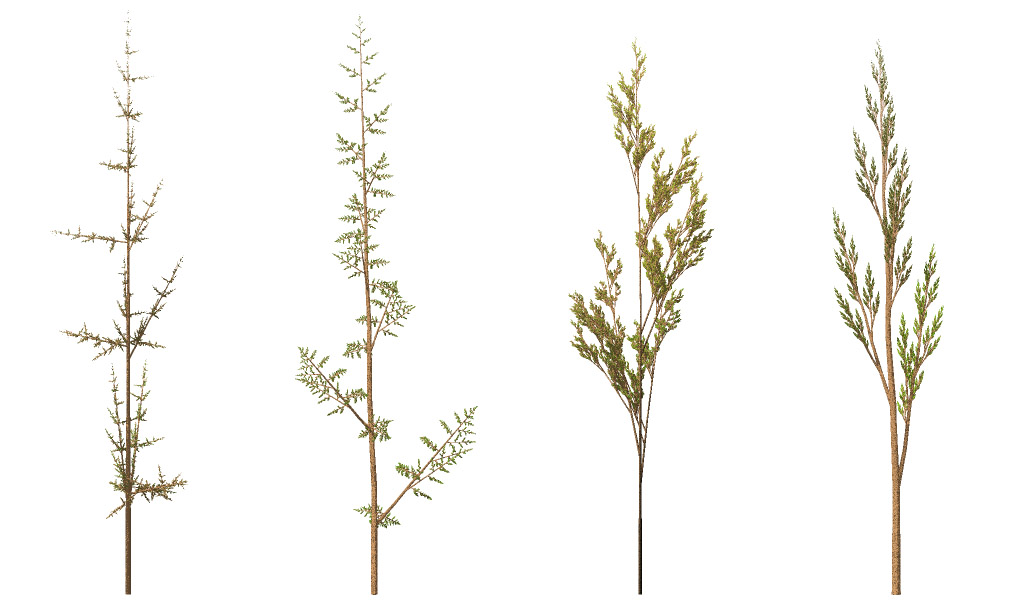
\includegraphics[scale=0.1]{images/exemple2D.png}
	\caption{Exemple d'arbre en 2D et 3D}
	\end{figure}

	\begin{figure}[h]
	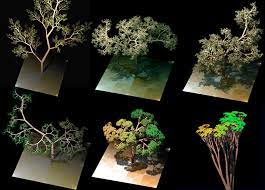
\includegraphics[scale=0.3]{images/exemple3D.png}
	\caption{source:https://en.wikipedia.org/wiki/L-system}
	\end{figure}
	\end{exampleblock}

\end{frame}


\section{Présentation des différentes interfaces}

\subsection{Le menu principale}

\begin{frame}

	\begin{block}{Le menu principale}

	\begin{figure}[h]
	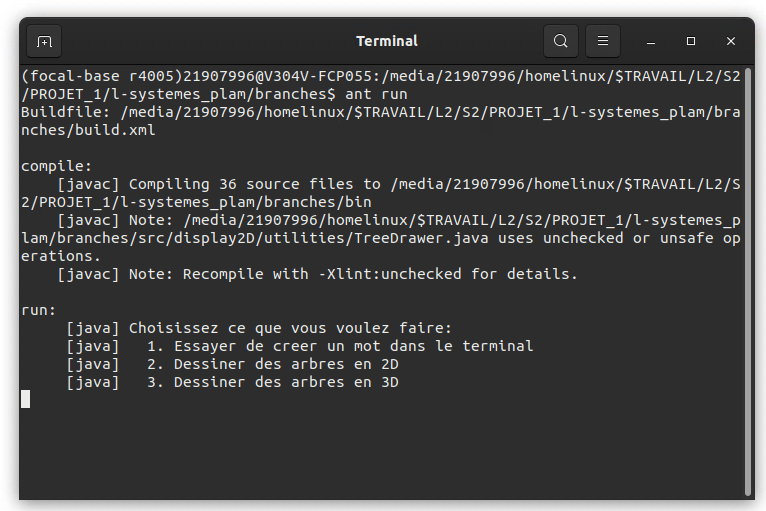
\includegraphics[scale=0.5]{images/menuPrincipale.png}
	\end{figure}

	\end{block}

\end{frame}


\subsection{En console}

\begin{frame}

	\begin{block}{Interpréteur en console}
	\begin{figure}[h]
	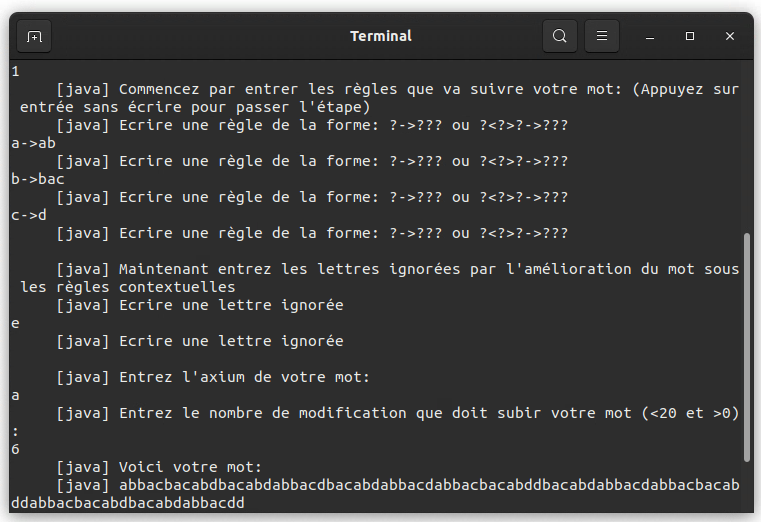
\includegraphics[scale=0.45]{images/treeConsole.png}
	\end{figure}

	\end{block}

\end{frame}

\subsection{Interface 2D}

\begin{frame}

	\begin{block}{Interpréteur en 2D}
	\begin{figure}[h]
	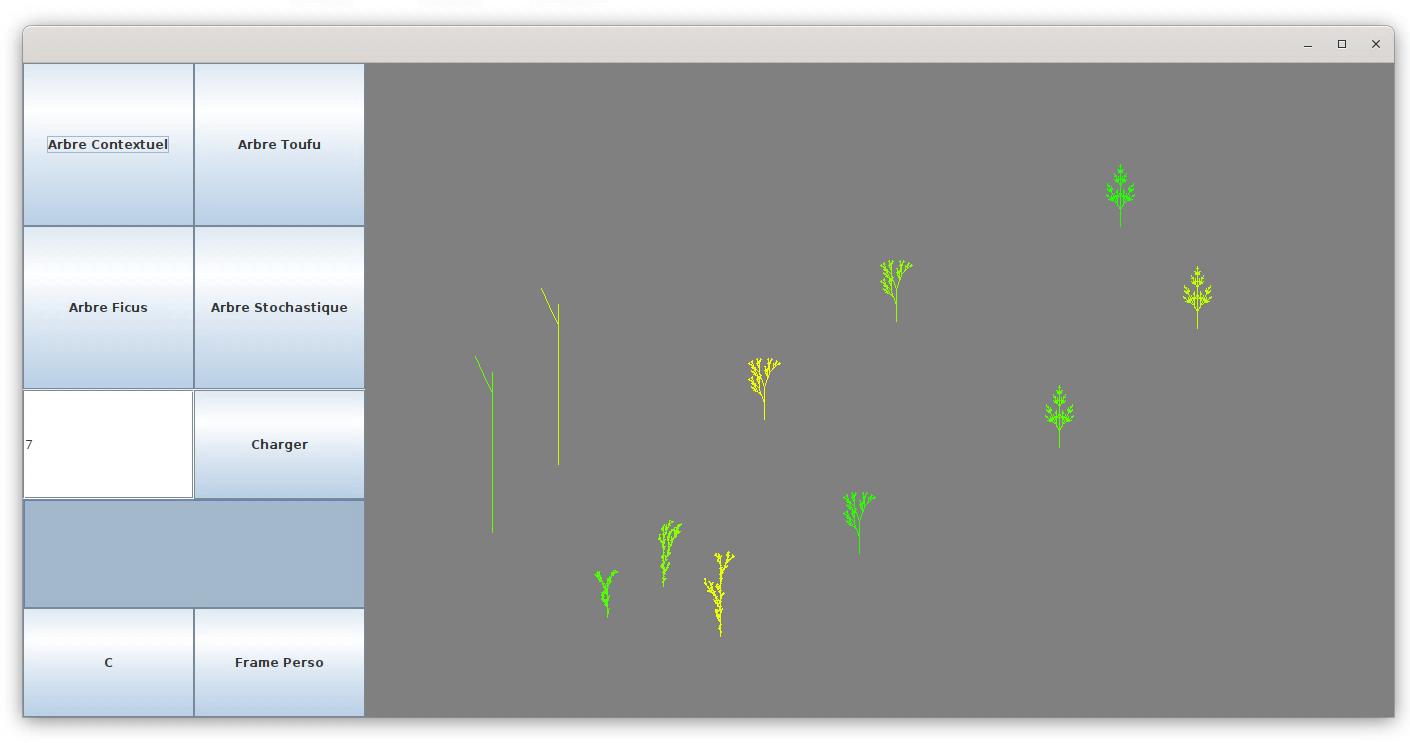
\includegraphics[scale=0.28]{images/interface2D.png}
	\end{figure}

	\end{block}

\end{frame}
\begin{frame}

	\begin{block}{Interface de personnalisation}
	\begin{figure}[h]
	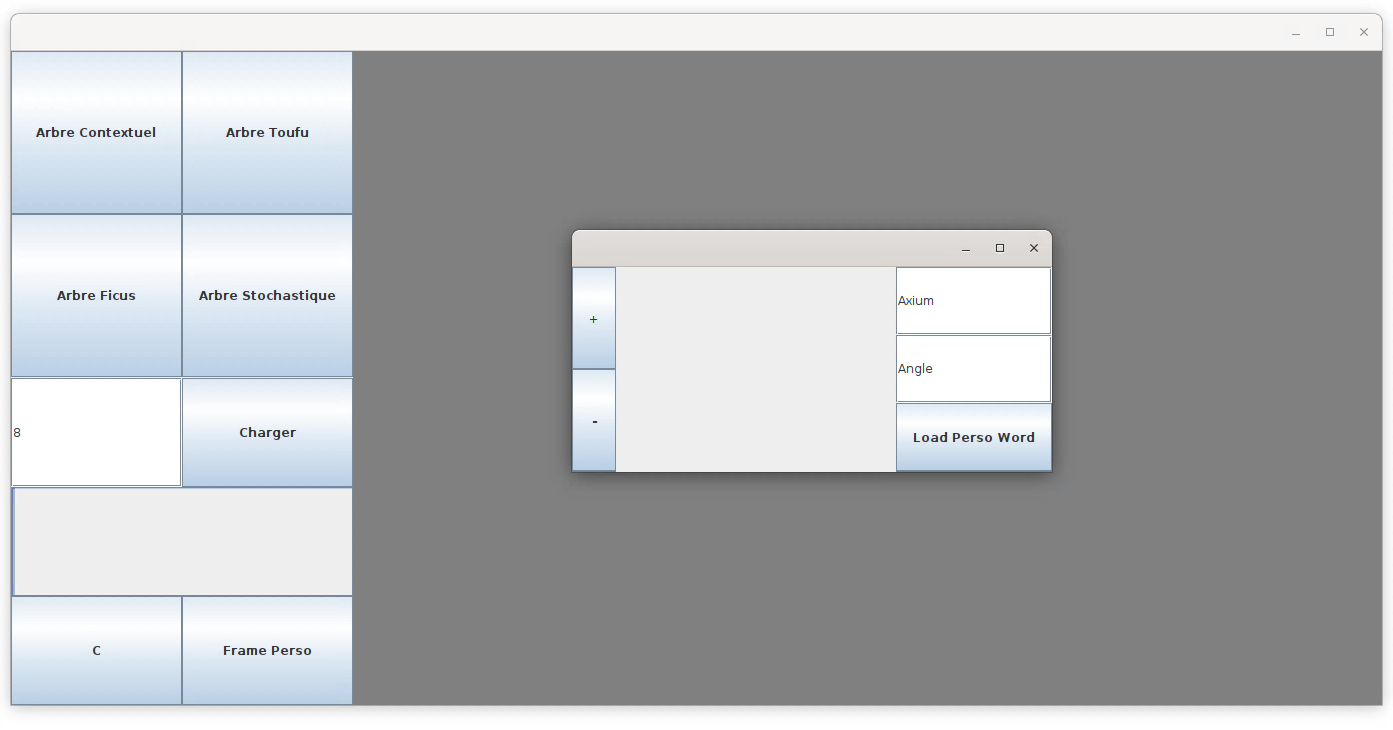
\includegraphics[scale=0.28]{images/interface2DPerso.png}
	\end{figure}

	\end{block}

\end{frame}
\subsection{Interface 3D}

\begin{frame}

	\begin{block}{Interpréteur en 3D}
	\begin{figure}[h]
	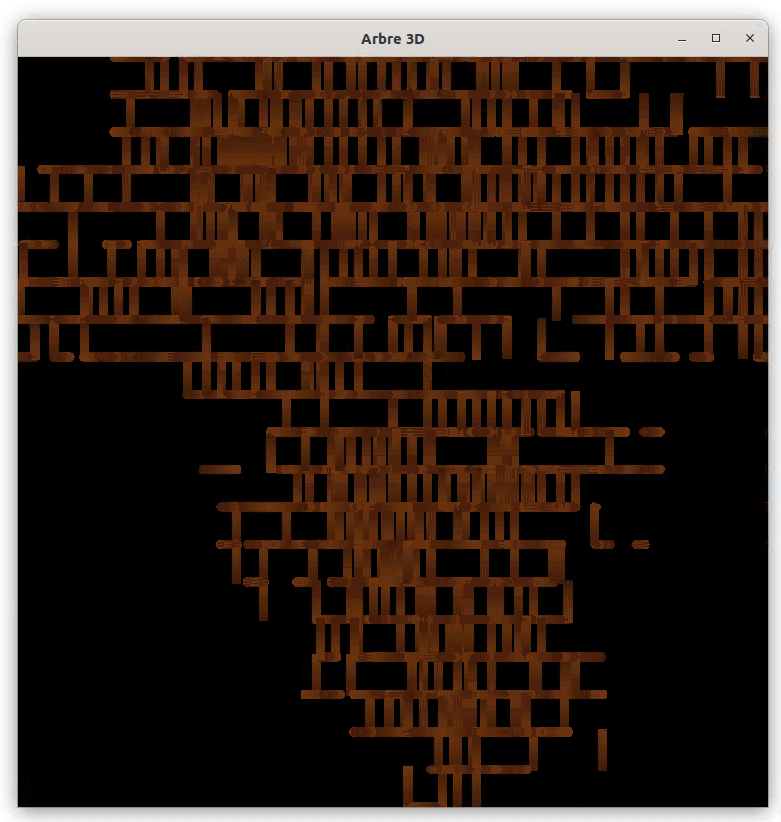
\includegraphics[scale=0.28]{images/interface3D.png}
	\end{figure}

	\end{block}

\end{frame}




\section{Les algorithmes importants}
\subsection{Le modèle}

\begin{frame}
	\begin{block}{Evolution d'un mot}

	\begin{figure}[h]
	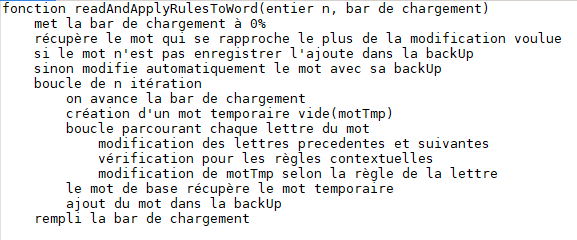
\includegraphics[scale=0.55]{images/readAndApply.png}
	\caption{L'algorithme readAndApply}
	\end{figure}
	

	\end{block}
\end{frame}




\subsection{Les dessins}

\begin{frame}

	\begin{block}{Dessin en 2D}

	\begin{figure}[h]
	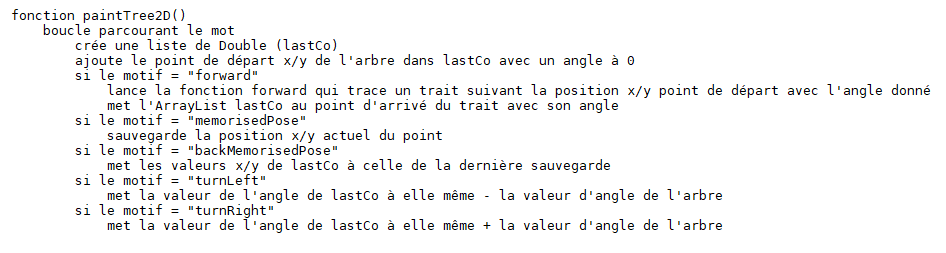
\includegraphics[scale=0.44]{images/paintTree2D.png}
	\caption{Algorithme permmettant de dessiner un arbre en 2D}
	\end{figure}

	\end{block}

\end{frame}
\begin{frame}

	\begin{block}{Dessin en 3D}

	\begin{figure}[h]
	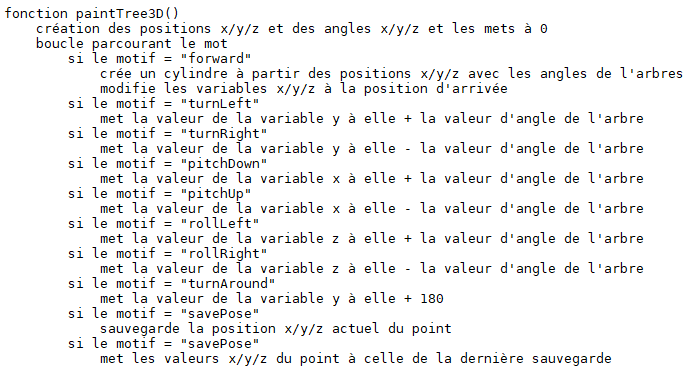
\includegraphics[scale=0.44]{images/paintTree3D.png}
	\caption{Algorithme permmettant de dessiner un arbre en 3D}
	\end{figure}

	\end{block}


\end{frame}



\subsection{Les threads}

\begin{frame}

	\begin{block}{Thread de la frame de personnalisation}

	\begin{figure}[h]
	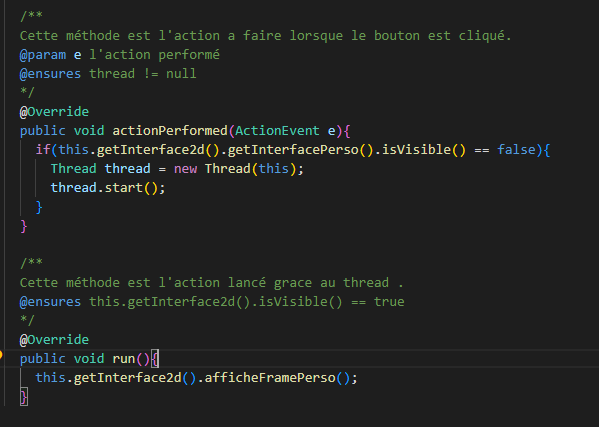
\includegraphics[scale=0.6]{images/interface2DPersoCode.png}
	\caption{Thread permettant d'afficher la framePersoi}
	\end{figure}

	\end{block}

\end{frame}

\begin{frame}
	\begin{block}{Thread du chargement d'un arbre}

	\begin{figure}[h]
	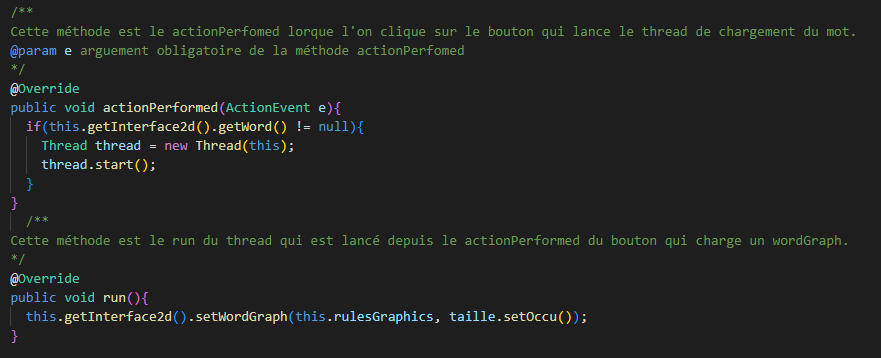
\includegraphics[scale=0.45]{images/loadTreeCode.png}
	\caption{Thread permettant de charger un arbre}
	\end{figure}

	\end{block}

\end{frame}
\section{Les tests}
\begin{frame}
	\begin{block}{Exemple de code de nos tests}

	\begin{figure}[h]
	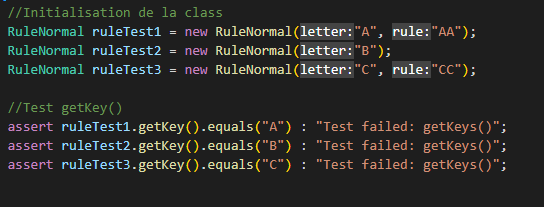
\includegraphics[scale=0.5]{images/testCode.png}
	\end{figure}

	\end{block}

\end{frame}

\begin{frame}
	\begin{block}{Résulats de nos tests}

	\begin{figure}[h]
	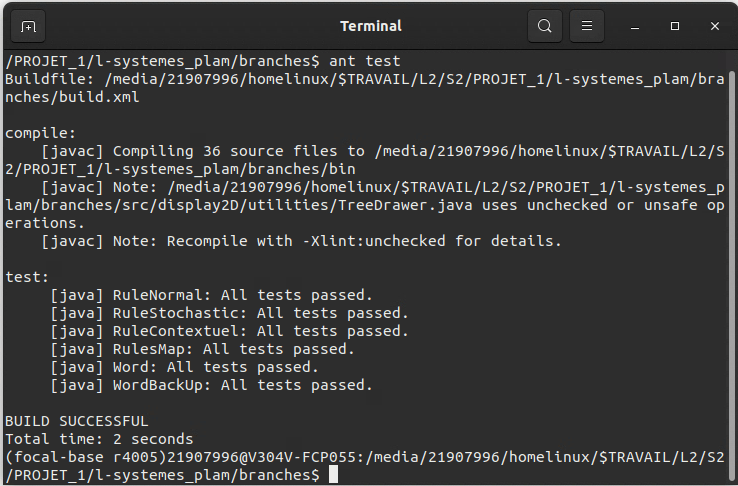
\includegraphics[scale=0.45]{images/ant_test.png}
	\end{figure}

	\end{block}

\end{frame}

\section{Conclusion}
\begin{frame}

\begin{block}{Les objectifs du projet}
	\begin{itemize}
		\item Les problèmes rencontrés et les points à améliorer
		\item Notre ressenti sur le projet
	\end{itemize}
\end{block}

\end{frame}

\end{document}
